\subcaptionbox{microscopig image}[.45\textwidth]{
\begin{tikzpicture}[baseline]
    \node[anchor=south east,inner sep=0] at (0,0) {
    \scalebox{-1}[1]{\includegraphics[width=0.45\textwidth, trim = 919 1205 1029 743, clip, interpolate=false, ]{data/Taorad_USAF_AB4_LB85_5pct_5ms_a00_t000_1.png}}};
\begin{scope}[xscale=-1]
    % \draw[magenta,ultra thick,rounded corners] (0.25,0.5) rectangle (1.5,1.25);
    \draw[magenta,ultra thick,dashed,rounded corners] (0.25,0.5) rectangle (1.4,1.175);
    % \draw[yellow,ultra thick,rounded corners] (2,0.75) rectangle (3.15,1.5);
    \draw[yellow,ultra thick,dashed,rounded corners] (1.85,0.8) rectangle (2.9,1.4);
    % \draw[cyan,ultra thick,rounded corners] (3.0,2.3) rectangle (3.9,2.8);
    \draw[cyan,ultra thick,dashed,rounded corners] (2.75,2.1) rectangle (3.6,2.6);
    % \draw[green,ultra thick] (0,0) grid (5,5);
\end{scope}
\end{tikzpicture}
\hfill}
\subcaptionbox{line plots. \itodo{single line plots not good}}[.45\textwidth]{
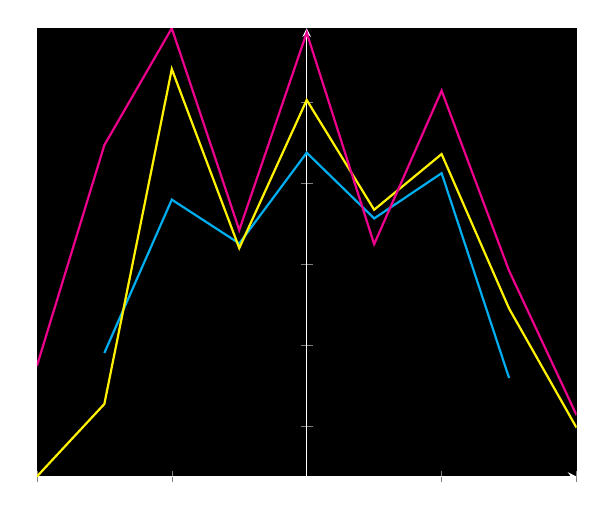
\begin{tikzpicture}[baseline]
\begin{axis}[%
axis x line = center,
axis y line = center,
xticklabels={,,},
yticklabels={,,},
scaled y ticks=false,
axis background/.style={fill=black},
axis line style={white},
]
\addplot [cyan, thick] coordinates {
(-3,	9530.667)
(-2,	19007.85)
(-1,	16297.67)
(0,	21909.00)
(1,	17846.71)
(2,	20642.69)
(3,	7984.000)
};
\addplot [yellow, thick] coordinates {
(-4,	1890.667)
(-3,	6374.111)
(-2,	27080.000)
(-1,	16011.000)
(0,	25166.666)
(1,	18383.334)
(2,	21824.000)
(3,	12277.556)
(4,	4910.222)
};
\addplot [magenta, thick] coordinates {
(-4,	8725.333)
(-3,	22378.074)
(-2,	29604.346)
(-1,	17126.518)
(0,	29328.791)
(1,	16255.111)
(2,	25744.297)
(3,	14614.123)
(4,	5688.889)
};
\end{axis}
\end{tikzpicture}
% \includegraphics[width=0.45\textwidth]{example-image}
}